\documentclass{article}
\usepackage{listings, xcolor, graphicx, inconsolata}
\setlength{\parindent}{0pt}

\definecolor{lgray}{rgb}{0.95, 0.95, 0.95}
\definecolor{lgray2}{rgb}{0.75, 0.75, 0.75}

\lstset{
  language=C++,
  aboveskip=10pt,
  belowskip=10pt,
  frame=leftline,
  xleftmargin=15pt,
  framexleftmargin=20pt,
  breaklines=true,
  basicstyle=\small,
  showstringspaces=false,
  backgroundcolor=\color{lgray},
  rulecolor=\color{lgray2},
  basicstyle=\ttfamily\footnotesize,
  keywordstyle=\color{blue},
  stringstyle=\color{red},
  commentstyle=\color{green},
  numbers=left,               
  numberstyle=\tiny\color{gray},
  stepnumber=1
}

\title{CS135; User-Defined Simple Data Types, Namespaces, and the
\texttt{string} Type}
\author{Gael Zarco}
\date{\today}

\begin{document}

\maketitle

C++ simple data types are split intro three categories:
\begin{enumerate}
  \item Integral
  \item Floating-point
  \item \texttt{enum}
\end{enumerate}

\begin{lstlisting}[caption={\texttt{namespace} Example}]
 using namespace std;
\end{lstlisting}

The above is used in every C++ program that follows the ANSI/ISO Standard C++
header files.

% SECTION 1 %
\section{Enumerations}
Data-types allow you to specify what values are legal and tell the user what
kinds of operations are allowed on those values. Enumerations allow you to
create simple data types.

\vspace{8pt}
The \textbf{Enumeration Type} requires the following:
\begin{enumerate}
  \item A name for the data type.
  \item A set of values for the data type.
  \item A set of operations on the values.
\end{enumerate}

\begin{lstlisting}[caption={Enumeration Syntax}]
  enum typeName {value1, value2, ...};
\end{lstlisting}

\begin{itemize}
  \item \texttt{value1, value2, ...} are indentifiers called
    \textbf{enumerators}.
  \item \texttt{enum} is a reserved word in C++.
  \item The values between the braces can have a specified order between them.
    \begin{itemize}
      \item This mean the enumeration type is an ordered set of values.
      \item The default value assigned to these enumerators starts at 0.
        Increments for every value thereafter.
    \end{itemize}
  \item The enumerators are \textbf{NOT} variables.
\end{itemize}

% SECTION 1.1 %
\subsection{Declaring Variables}
Once a data type is defined, you can declare variables of that type.

\begin{lstlisting}[caption={\texttt{enum} Variable Declaration Syntax}]
  dataType identifier, identifier, ...; 

  \\ Example
  enum sports {BASKETBALL, FOOTBALL, SOCCER, BASEBALL, VOLLEYBALL};
\end{lstlisting}

The following statement declares \texttt{popularSport} and \texttt{mySport} to
be of type \texttt{sports}.

% SECTION 1.2 %
\subsection{Assignment}
Once the var is declared, you can store values in it.

\begin{lstlisting}[caption={\texttt{enum} Variable Assignment}]
  popularSport = FOOTBALL;

  // Copy the value of popularSport to mySport
  mySport = popularSport;
\end{lstlisting}

% SECTION 1.3 %
\subsection{Operations on Enumeration Types}
No arithmatic operations are allowed on the enumeration type. This includes the
increment and decrement operator. Use a cast when necessary:

\begin{lstlisting}[caption={\texttt{enum} Cast Example}]
  popularSport = static_cast<sports>(popularSport + 1);
\end{lstlisting}

This statement advances the the value of \texttt{popularSport} to the next
value in the list.

% SECTION 1.4 %
\subsection{Relational Operators}
Because an enumeration is ordered, relational operators can be used.

\begin{lstlisting}[caption={Enumeration Type Relational Operator Example}]
  FOOTBALL <= SOCCER    \\ true
\end{lstlisting}

% SECTION 1.5 %
\subsection{Enumeration Types and Loops}
Enumeration type is an integral type and can be used to increment, decrement,
and compare the values of the enumeration type (using cast).

\begin{lstlisting}[caption={Enumeration Type Loop}]
  for (mySport = BASKETBALL; mySport <= VOLLEYBALL; mySport = 
    static_cast<sports>(mySport + 1))
\end{lstlisting}

% SECTION 1.6 %
\subsection{Input/Output of Enumeration Types}
The enumeration type cannot be used for neither input or output (directly).

% SECTION 1.7 %
\subsection{Functions and Enumeration Types}
The enumeration type can be passed as a param to funcs by value or reference.
Funcs can also return a value of the enum type.

\begin{lstlisting}[caption={\texttt{enum} Types in Functions}]
  void printEnum(courses registered) {
    switch (registered) {
    case ALGEBRA:
    cout << "Algebra";
    break;
    case ANALYSIS:
    cout << "Analysis";
    break;
    case BASIC:
    cout << "Basic";
    break;
    case CHEMISTRY:
    cout << "Chemistry";
    break;
    case CPP:
    cout << "CPP";
    break;
    case HISTORY:
    cout << "History";
    break;
    case PYTHON:
    cout << "Python";
    break;
    case PHILOSOPHY:
    cout << "Philosophy";
    }    //end switch
  }      //end printEnum
\end{lstlisting}

% SECTION 1.8 %
\subsection{Declaring Variables When Defining the Enumeration Type}
\begin{lstlisting}[caption={Simultaneous \texttt{enum} Declaration and Variable
Declaration}]
  enum grades {A, B, C, D, F} courseGrade;
\end{lstlisting}

This listing defines an enumeration type, \texttt{grades} and declares a
variable \texttt{courseGrade} of type \texttt{grades}.

% SECTION 1.9 %
\subsection{Anonymous Data Types}
A data type where you directly specify values in the variable declaration with
no type name is called an \textbf{Anonymous Type}.
\begin{lstlisting}[caption={Anonymous Enumeration Type Example}]
  // No name is given to the data type
  enum {BASKETBALL, FOOTBALL, BASEBALL, HOCKEY} mySport;
\end{lstlisting}

Drawbacks:
\begin{enumerate}
  \item Anonymous data types cannot be passed as params to a func and a func can
    not return an anonymous data type.
  \item Values used in one anon data type can be used in a separate anon data
    type, but variables of those types are treated differently.
\end{enumerate}

\begin{lstlisting}[caption={illegal \texttt{enum} operations}]
  enum {english, french, spanish, german, russian} languages;
  enum {english, french, spanish, german, russian} foreignlanguages;

  languages = foreignlanguages;    // illegal
\end{lstlisting}

% SECTION 1.10 %
\subsection{\texttt{typedef} Statement}
You can create synonyms or aliases to a previously defined data type by using
the \texttt{typedef} statement.

\begin{lstlisting}[caption={\texttt{typedef} Statement Syntax}]
  typedef existingTypeName newTypeName;
\end{lstlisting}

\begin{itemize}
  \item \texttt{typedef} is a reserved word.
    \begin{itemize}
      \item Does not create any new data type; only creates an alias to the
        existing type.
    \end{itemize}
\end{itemize}

% SECTION 2 %
\section{Namespaces}
When a header file such as \texttt{iostream} is included in the program, the
global identifiers in the header file also become global identifiers in the
program.

\begin{itemize}
  \item This means that the compiler may return a syntax error if a global
    identifier is redefined.
  \item Third-party libraries and other software usually add a special character
    to the beginning of their global identifiers to avoid compiler errors.
    \begin{itemize}
      \item Do not do this in your own code.
    \end{itemize}
\end{itemize}

ANSI/ISO Standard C++ tries to solve this problem of overlapping identifiers
with the \texttt{namespace} mechanism.

\begin{lstlisting}[caption={\texttt{namespace} Statement Syntax}]
  namespace namespace_name {
    members
  }
\end{lstlisting}

Where \texttt{members} is usually named constants, variable declarations,
functions or another \texttt{namespace}.

\begin{itemize}
  \item \texttt{namespace} is a reserved word.
\end{itemize}

\begin{lstlisting}[caption={\texttt{namespace} Example}]
  namespace globalType {
    const int N = 10;
    const double RATE = 7.50;
    int count = 0;
    void printResult();
  }
\end{lstlisting}

This listing defined \texttt{globalType} to be a \texttt{namespace} with four
members with their respective types.

\begin{itemize}
  \item The scope of a \texttt{namespace} member is local to \texttt{namespace}.
\end{itemize}

To use a \texttt{namespace} member, you may:

\begin{enumerate}
  \item Use \texttt{namespace::identifier} (scope resolution operator).
  \item Use a \texttt{using} statement.
\end{enumerate}

\begin{lstlisting}[caption={\texttt{using} Statement Syntax (Two Ways)
}]
  using namespace namespace_name;

  using namespace::identifier;
\end{lstlisting}

% SECTION 3 %
\section{\texttt{string} Type}
The \texttt{string} type is a programmer-defined type and is not part of the C++
language; The C++ standard library supplies it. Therefore you must include the
header file in your program.

\begin{lstlisting}[caption={\texttt{string} Type Example}]
  string name = "Gael Zarco":
\end{lstlisting}

\begin{itemize}
  \item Strings are sequences of zero or more characters, therefore each
    charcter has an assigned position starting with 0 (0, 1, 2, etc.).
  \item Strings can store just about any size string. 
  \item The binary \texttt{+} operator and the array index (subscript) 
    \texttt{[]} operator are defined operations for strings.
\end{itemize}

The \textbf{Array Subscript Operator} resembles \texttt{[]} and can be used to
access a position of a character within a string.

\begin{lstlisting}[caption={Indexing Into A \texttt{string}}]
  string str1 = "Hello there";

  // Strings begin at index 0, 6 affects the 5th char
  str1[6] = 'T';
\end{lstlisting}

% SECTION 3.1 %
\subsection{Additional \texttt{string} Operations}

\begin{itemize}
  \item \texttt{string} has a data type \texttt{string::size\_type}.
  \item \texttt{string} has a named constant \texttt{string::npos}.
\end{itemize}

\begin{tabular}{|l|p{8.3cm}|}
\hline
\texttt{string::size\_type} & An unsigned integer (data) type \\ \hline
\texttt{string::npos} & The maximum value of the (data) type \texttt{string::size\_type}, a number such as \texttt{4294967295} on many machines \\ \hline
\end{tabular}

\vspace{8pt}
There are many other functions for string manipulation:

\begin{center}
    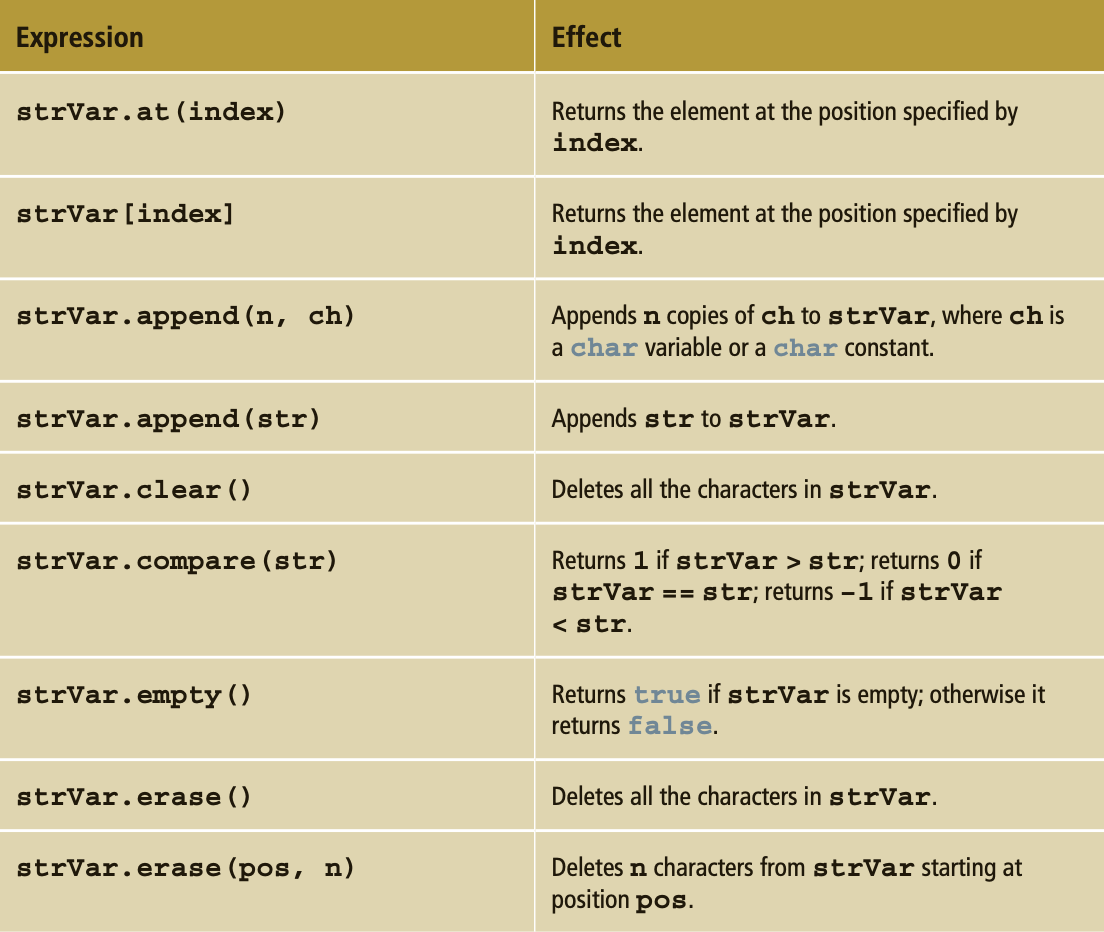
\includegraphics[width=0.9\textwidth]{str-funcs-1.png}
    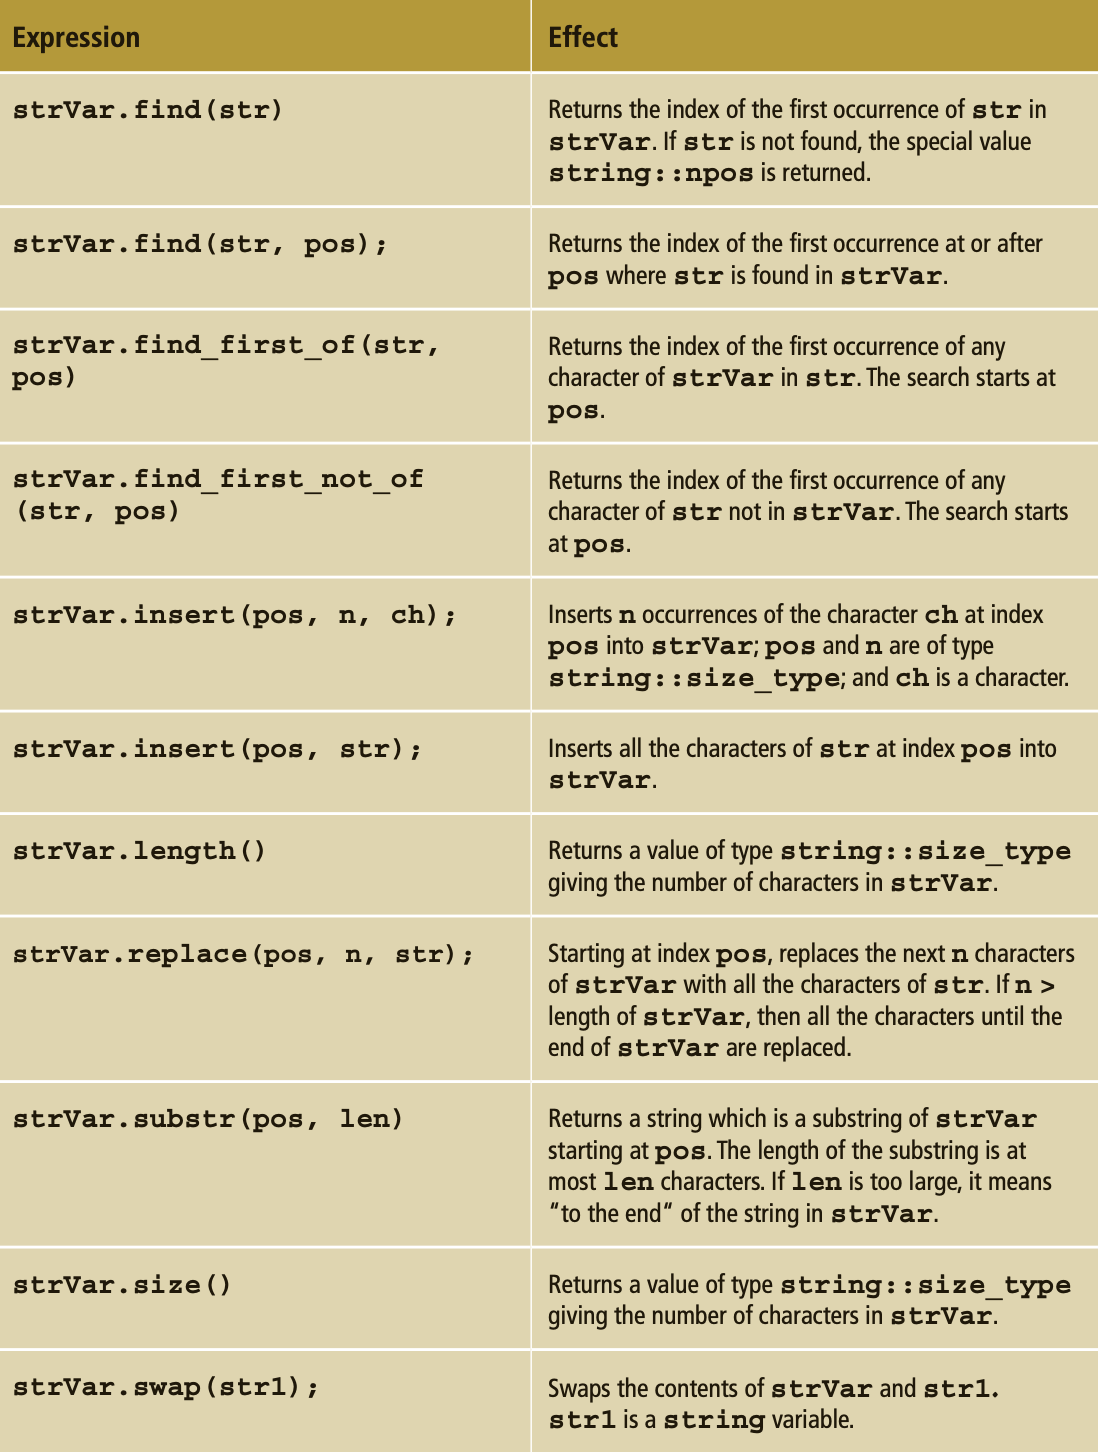
\includegraphics[width=0.9\textwidth]{str-funcs-2.png}
\end{center}

\end{document}
